\documentclass[12pt,a4paper]{article}
\usepackage[utf8]{inputenc}
\usepackage{amsmath}
\usepackage{amsfonts}
\usepackage{amssymb}
\usepackage{lipsum}
\usepackage{textcomp}

\usepackage{makecell} % linebreak dans une cellule
\usepackage{multicol} % twocols localement
\usepackage{vwcol} % idem mais avec largeur variable
\usepackage{color, colortbl} % colorer les tableaux
\usepackage{enumitem} % utiliser des lettres pour énumérer
\usepackage{wrapfig} % insérer des images dans dutexte

% --- geometry ---
\usepackage{geometry}
\geometry{legalpaper, margin=2cm}
% ---

% --- xcolor ---
\usepackage{xcolor}
\definecolor{lightgray}{gray}{0.9}
% ---

% --- tcolorboxes ---
\usepackage[most]{tcolorbox}
\newtcolorbox{definition}[2][]{%
  attach boxed title to top left
               = {yshift=-8pt},
  colback      = white,
  colframe     = gray,
  fonttitle    = \bfseries,
  colbacktitle = gray,
  title        = #2,#1,
  enhanced,
}
% ---

\author{Paul Clavier}
\title{Chapitre 1 - Tableaux et graphiques}

\begin{document}

% --- Section & subsection renum ---
\renewcommand\thesection{\Roman{section}}
\renewcommand\thesubsection{\arabic{subsection}}
% ---


\begin{center}
	\fbox{\huge Chapitre 1 - Tableaux et graphiques}
\end{center}

\section{Tableaux}

\begin{definition}{Règle}
Un tableau permet de regrouper et d’organiser des données, de lire facilement des informations

Pour lire une information correspondante à une case, on croise les informations données à la fois par la ligne et la colonne correspondante à cette case.
\end{definition}

\textbf{Exemple:} Les tableaux ci-dessous sont des tableaux à simple entrée.

\begin{multicols}{2}
\begin{tabular}{|c|c|}
\hline \rowcolor{lightgray}
Continent & \thead{Population en 1995\\en millions d'habitants} \\ \hline
Afrique & 728 \\ \hline
Asie & 3 458 \\ \hline
Europe & 727 \\ \hline
Amérique latine & 482 \\ \hline
Amérique du Nord & 293 \\ \hline
Océanie & 28 \\ \hline
\end{tabular}

\begin{tabular}{|c|c|}
\hline \rowcolor{lightgray}
Continent & \thead{Population en 2008\\en millions d'habitants} \\ \hline
Afrique & 987 \\ \hline
Asie & 4 075 \\ \hline
Europe & 731 \\ \hline
Amérique latine & 579 \\ \hline
Amérique du Nord & 342 \\ \hline
Océanie & 35 \\ \hline
\end{tabular}
\end{multicols}

\begin{enumerate}[label=\textbf{\alph*.}]
\item Que signifient les nombres 727 et 35 ? \\
Le nombre  727  indique qu'il y avait 727 millions d'habitants en 1995 en Europe.\\
Le nombre  35  indique qu'il y avait 35 millions d'habitants en 2008 en Océanie.
\item Fusionne ces deux tableaux pour n'en faire qu'un seul à double entrée.
\end{enumerate}

%\begin{vwcol}[widths={0.7, 0.2}]
\begin{minipage}{0.7\textwidth}
\begin{tabular}{|c|c|c|}
\hline \rowcolor{lightgray}
Continent & \thead{Population en 1995\\en millions d'habitants}& \thead{Population en 2008\\en millions d'habitants} \\ \hline
Afrique & 728 & 987 \\ \hline
Asie & 3 458 & 4 075 \\ \hline
Europe & 727 & 731 \\ \hline
Amérique latine & 482 & 579 \\ \hline
Amérique du Nord & 293 & 342 \\ \hline
Océanie & 28 & 35 \\ \hline
\end{tabular}
\end{minipage}
\begin{minipage}{0.3\textwidth}
\textbf{Remarque:} Un seul tableau permet d'effectuer des comparaisons facilement et rapidement. \\
On remarque, par exemple, que la population a augmenté entre 1995 et 2008 et ce, dans chacun des continents.
\end{minipage}
%\end{vwcol}

\section{Représentations graphiques et interprétations}

\subsection{Diagramme en bâton}

\begin{definition}{Règle}
Dans un diagramme en bâton, les hauteurs des bâtons sont proportionnelles aux quantités représentés.
\end{definition}

\begin{wrapfigure}{r}{0.45\textwidth}
\vspace{-30pt}
  \begin{center}
	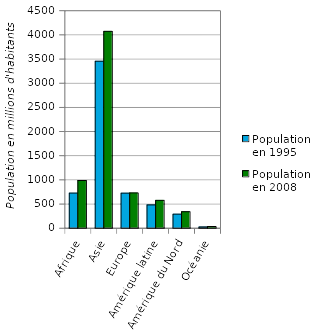
\includegraphics[scale=0.85]{img/diag-bat.png}
  \end{center}
 \vspace{-120pt}
\end{wrapfigure}

\textbf{Exemple:} Ci-contre, on a construit un diagramme en barres représentant la population en 1995 et en 2008, en millions d'habitants, par continent.

\textbf{Question:} Quel est le continent où il y a le plus d'écart entre la population en 1995 et celle en 2008 ?

\textbf{Réponse:} C'est en Asie que l'écart entre la population en 1995 et celle en 2008 est le plus grand.

\newpage
\subsection{Diagramme circulaire, semi-circulaire}

\begin{definition}{Règle}
Dans un diagramme circulaire (ou semi-circulaire), les mesures des angles sont proportionnelles aux quantités représentées. 
\end{definition}

\begin{wrapfigure}{r}{0.45\textwidth}
\vspace{-30pt}
  \begin{center}
	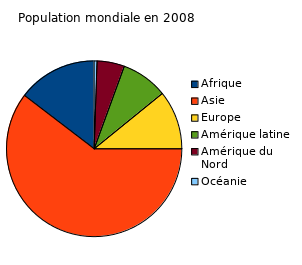
\includegraphics[scale=0.95]{img/diag-camb.png}
  \end{center}
\vspace{-40pt}
\end{wrapfigure}

\textbf{Exemple:} Ci-contre, on a construit un diagramme circulaire représentant la population en 2008, en millions d'habitants, par continent.

\begin{enumerate}[label=\textbf{\alph*.}]
\item Classe les cinq continents du moins peuplé au plus peuplé en 2008.
\item Est-il vrai que plus de la moitié de la population mondiale en 2008 se trouve en Asie ?
Justifie.
\end{enumerate}

\begin{enumerate}[label=\textbf{\alph*.}]
\item Pour classer les continents du moins peuplé au plus peuplé en 2008, il suffit de comparer les mesures des angles de couleur et on obtient :
Océanie, Amérique du Nord, Amérique latine, Europe, Afrique et Asie.
\item Oui, plus de la moitié de la population mondiale en 2008 se trouve en Asie car l'angle du secteur orange mesure plus de 180°.
\end{enumerate}

\subsection{Graphique cartésien}

\begin{definition}{Règle}
Un graphique cartésien permet de représenter l'évolution d'une grandeur en fonction d'une autre.
\end{definition}

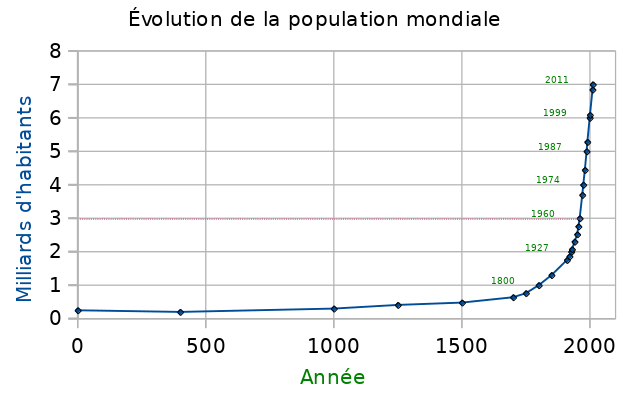
\includegraphics[scale=1]{img/graph-cart.png} 

\begin{enumerate}[label=\textbf{\alph*.}]
\item En quelle année les 3 milliards d'habitants ont étés atteints?\\
On peut lire que les 3 milliards d'habitants ont étés atteins en 1960.
\item Combien y avait-il d'habitants dans le monde en 2000?\\
En 2000, il y avait environ 6 milliards d'habitants.
\end{enumerate}

\end{document}